\scanpage{162}
% archive sheet number: 161
% L1-2, in the orientation of the scan
injectif, alors les $H^q_J(N)$ sont nuls pour $q>0$, et $H^0_J(N)$ est injectif, OK \unsure{----}

% The remaining writing is sideways on the scan; transcribed in its reading direction.
% T1: upper cancelled table
\deleted{Ind pro}
\[
\underline{\operatorname{Ext}}^{\unsure{i|1}}(F,G)
\]
\diagram{$\deleted{\begin{array}{c|c|c|c|c|c|c|c|c|c}
\underline{\operatorname{Hom}}(F,G)&\mathbb Z/\unsure{\ell|l}\mathbb Z&\unsure{\mathbb Z/p\mathbb Z}&{\unsure{\mu|H}}_p&\alpha_p&{\unsure{\mathbb G|G}}_m&\mathbb G_a&\unsure{\mathbb V|V}&\unsure{\mathbb Z|A}&A\\\hline
\mathbb Z/\ell\mathbb Z&\mathbb Z/\ell\mathbb Z&&0&0&\mu_\ell&0&0&0&{}_{\ell}A\\\hline
\mu_p&0&&\mathbb Z/p\mathbb Z&&&&&&
\end{array}}$}

% T2: heading and abandoned heading
Tableau des \uline{Hom}

\deleted{$\mu_p\quad\alpha_p\quad\mathbb Z/p\mathbb Z\quad\mathbb Z/\ell\mathbb Z$ Tableau des $\underline{\operatorname{Ext}}$}

% D1: small matrix, above the right corner of the main table
\diagram{$\left(\begin{array}{ccc}
\mathbb Z/p\mathbb Z&0&0\\
\alpha_p&\mathbb G_a&0\\
\mu_p&\alpha_p&\mathbb Z/p\mathbb Z
\end{array}\right)$}

% T3: main table. Blank cells in T1 are blank in the manuscript.
\diagram{$\begin{array}{c|c|c|c|c|c|c|c|c|c}
&\mathbb Z/\ell\mathbb Z&\mathbb Z/p\mathbb Z&\alpha_p&\mu_p&\mathbb G_m&\mathbb G_a&\mathbb Z&\mathbb V&A\\\hline
\mathbb Z/\ell\mathbb Z&\mathbb Z/\ell\mathbb Z&0&0&0&\mu_\ell&0&0&0&{}_{\ell}A\\\hline
\mathbb Z/p\mathbb Z&0&\mathbb Z/p\mathbb Z&\alpha_p&\mu_p&\mu_p&\mathbb G_a&0&\mathbb V&{}_{p}A\\\hline
\alpha_p&0&0&\mathbb G_a&\alpha_p&\alpha_p&\mathbb G_a&0&\text{\tikz[baseline=(c.base)]{\node[draw,rounded corners=6pt,inner sep=2pt] (c) {$\unsure{\text{gros}|\text{quoi}}?$};}}&\deleted{\unsure{\mathbb V}({\unsure{t}}_A^{\unsure{1-p|1/p}})}\ {?}\\\hline
\mu_p&0&0&0&\mathbb Z/p\mathbb Z&\mathbb Z/p\mathbb Z&0&0&0\deleted{\unsure{?}}&\deleted{({\unsure{t}}_A^{p})_{\unsure{k}}}\ {?}\\\hline
\mathbb G_m&0&0&0&0&\mathbb Z&0&0&0&0\\\hline
\mathbb G_a&0&0&\text{\tikz[baseline=(c.base)]{\node[draw,rounded corners=6pt,inner sep=2pt] (c) {$\unsure{\text{gros}|\text{quoi}}$};}}&\mathbb V&\mathbb V&\boxed{\begin{gathered}\deleted{\unsure{\mathbb G_a}}\\{\unsure{\text{Imm}}}^{\unsure{2}}\end{gathered}}&0&\text{\tikz[baseline=(c.base)]{\node[draw,rounded corners=6pt,inner sep=2pt] (c) {$\mathbb G_a?$};}}&\unsure{\text{gros}}\\\hline
\mathbb Z&\mathbb Z/\ell\mathbb Z&\mathbb Z/p\mathbb Z&\alpha_p&\mu_p&\mathbb G_m&\mathbb G_a&\mathbb Z&\mathbb V&A\\\hline
\mathbb V&0&0&\mathbb G_a&\deleted{\unsure{\mathbb G}}\mathbb G_a&\mathbb G_a&\text{\tikz[baseline=(c.base)]{\node[draw,rounded corners=6pt,inner sep=2pt] (c) {$\mathbb G_a$};}}\unsure{!}&0&\text{\tikz[baseline=(c.base)]{\node[draw,rounded corners=6pt,inner sep=2pt] (c) {$\unsure{\text{Imm}}$};}}&\underline{V}(\omega_A)\\\hline
A&0&0&0&0&0&0&0&0?&\mathbb Z^{\unsure{n|m}}
\end{array}$}
% margin note written sideways
\margin{\unsure{con|conn}\ $\left\{\begin{array}{c}\alpha_p\\\mu_p\\\mathbb G_m\\\mathbb G_a\end{array}\right.$}
% margin note written sideways
\margin{$\underline{\operatorname{Hom}}(\alpha_p,\mathbb G_m)$}
% margin note written sideways
\margin{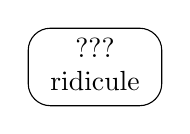
\begin{tikzpicture}\node[draw,rounded corners=8pt,inner sep=2pt] {\begin{tabular}{c}???\\\unsure{ridicule}\end{tabular}};\end{tikzpicture}}
